\documentclass[../main.tex]{subfiles}
\usepackage[english]{babel}
\graphicspath{{\subfix{../images}}}
\usepackage{lipsum}
\begin{document}

The results achieved with the different training strategies are reported in the following sections.
They are divided according to the related datset.

\section{Results on Deepskin}
\subsection{EfficientNet}

In table \ref{tab:results-eff-deepskin} we report the number of images used for the training and for the validation, the number of correctly segmented validation images (according to the expert evaluation), and the metric scores achieved (on the validation set) after 150 epochs for each round of training, respectively. 
The percentages of training and validation images are referred to the splitting of labelled data, performed at each round. 
The percentage of correct segmentation is  referred to the whole set of available samples, i.e. 1564 images.
The metric scores are calculated on validation images, which were correctly segmented the previous round. 
Such score are ensuring the model performances among the rounds and we expect them to be almost constant.
\hspace{-1cm}
\begin{table}[H]
    \centering
    \begin{tabular}{c|c|c|c|c|}
 
        \textbf{} & \textbf{Round 1} & \textbf{Round 2} & \textbf{Round 3} & \textbf{Round 4 } \\ \hline
        \textbf{N° training images} & 130 (89.7\%) & 331 (89.9\%) & 824 (90\%) & 1228 (90\%)\\ \hline
        \textbf{N° validation images} & 15 (11.3\%) & 37 (19.1\%) & 92 (10\%) & 137 (10\%)  \\ \hline
        \textbf{N° correct segmentation} &  368 (24\%) & 916 (59\%) & 1365 (87\%) & 1477 (94\%)  \\ \hline
        \textbf{DSC metric} & 0.95 & 0.98 & 0.97 & 0.96  \\ \hline
        \textbf{Precision metric} & 0.93 & 0.98 & 0.97 & 0.96  \\ \hline
        \textbf{Recall metric} & 0.96 & 0.98 & 0.97 & 0.96  \\ \hline
    \end{tabular}
    \caption{Results obtained by the EfficientNet model using the active semi-supervised learning procedure at each round.
    The percentages of training and validation images are referred to the splitting of labelled data, performed at each round. 
The percentage of correct segmentation is  referred to the whole set of available samples, i.e. 1564 images.
The metric scores are calculated on validation images, which were correctly segmented the previous round. 
Such score are ensuring the model performances among the rounds and we expect them to be almost constant.} 
    \label{tab:results-eff-deepskin}
\end{table}

The training procedure of the fourth round with an evolution of the average metrics along the training epochs (150) is showed in Figure \ref{fig:eff-deepskin-train}. The metrics are calculated on the validation set which composes 10\% of images.
In the same figure, a predicted segmentation of an image among the Deepskin dataset is also reported.

\begin{figure}[H] 
\begin{center}
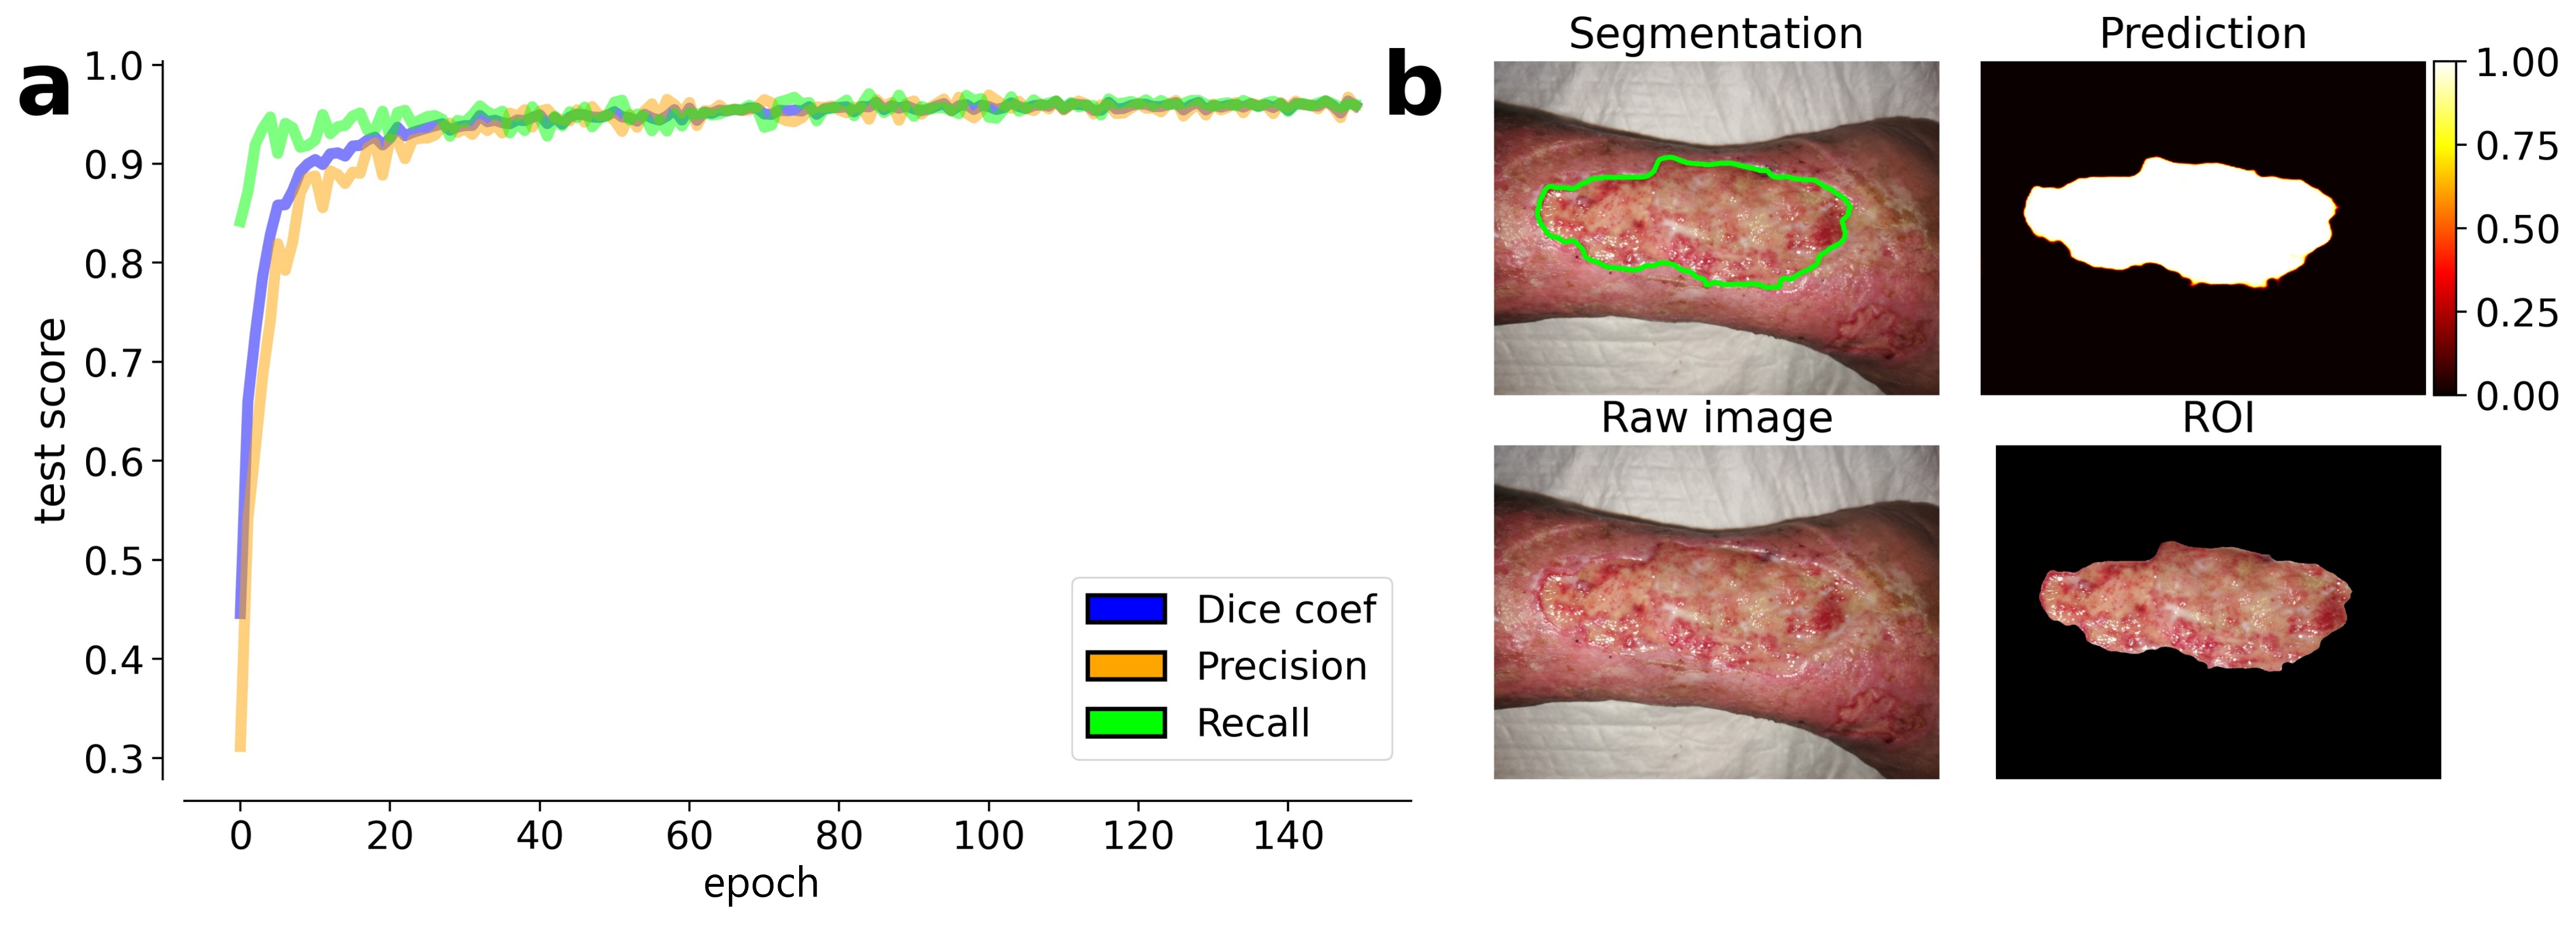
\includegraphics[width=16cm]{images/eff-train-deepskin.png}
\caption{\small{Results obtained by the trained U-Net model at the fourth round of training. (a) Evolution of the average metrics (Dice coefficient, Precision, and Recall) along the training epochs (150). The metric values are estimated on the validation set, i.e. the 10\% of available images, which were excluded from the training set. (b) On the top-left the resulting segmentation. On the top-right the predicted segmentation mask. On the bottom-left the raw (input) image. On the bottom-right the resulting ROI of the wound area.}}\label{fig:eff-deepskin-train}
\end{center}
\end{figure}

\subsection{MobileNet}

The MobileNet model was trained on the 1477 correctly segmented images. The labels, predicted at the fourth round of ASSL with EfficientNet, were used as ground trouth for the training procedure.
In Figure \ref{fig:mob-deepskin-train} we report the score evaluations of BF loss function, IoU and $F_1$ metrics after 100 training epochs. 
The metric values are estimated on the validation set, i.e. 10\% of available images, which were excluded from the training set.

\begin{figure}[H] 
\begin{center}
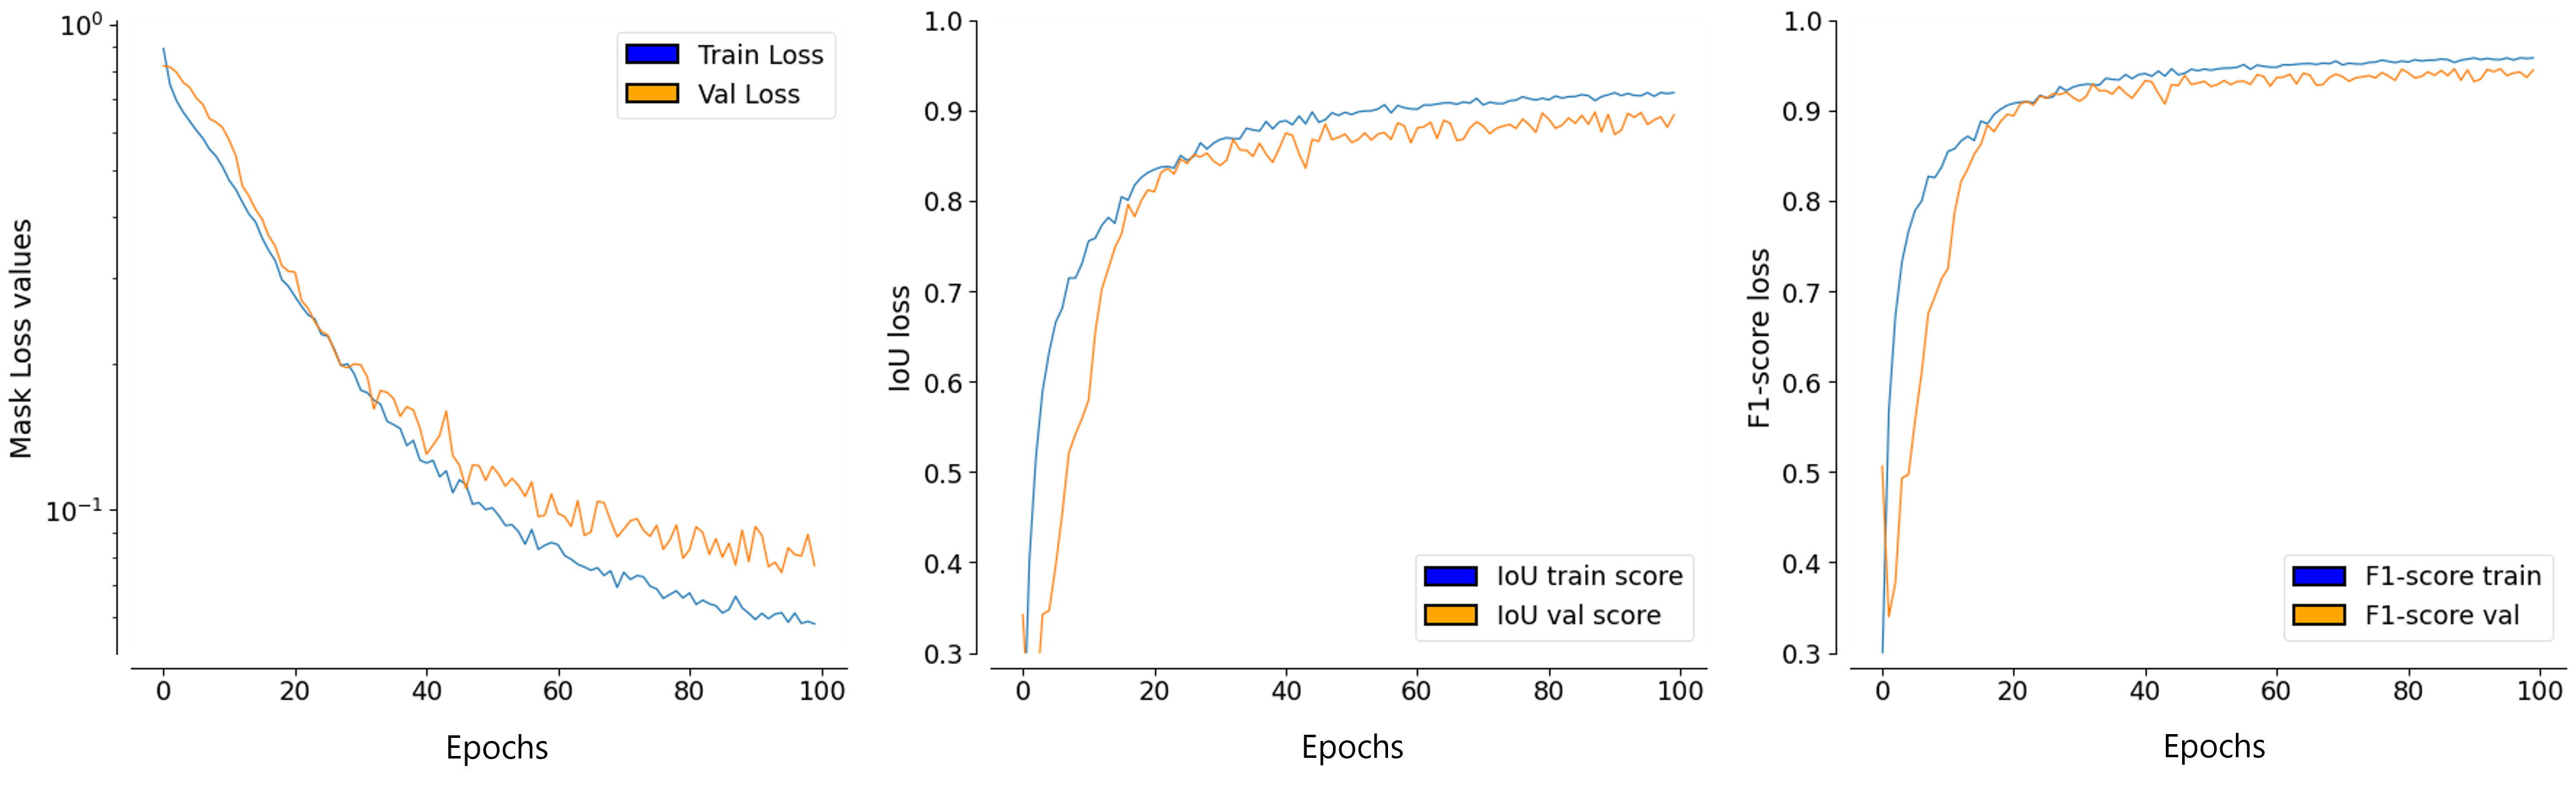
\includegraphics[width=16cm]{images/mob-train-deepskin.png}
\caption{\small{Evolution of the average metrics (BF loss, $F_1$ and IoU) along the training epochs (100).
We report the calculation on both training and validation set to ensure the absence of over fitting effects. }}\label{fig:mob-deepskin-train}
\end{center}
\end{figure}

The MobileNet model shows high capability of learning the wound segmentation task. 
The best scores results, calculated on the validation set, are reported in Table \ref{tab:results-mob-deepskin}.
\begin{table}[H]
    \centering
    
    \begin{tabular}{|l|l|}
    \hline
         IoU  & $F_1$  \\ \hline
         0.89 & 0.94 \\ \hline
    \end{tabular}
    \caption{Results obtained by the MobileNet model trained on the masks segmented by EfficientNet, we show metrics scores achieved (on the validation set, excluded from training) after 100 epochs.
   }\label{tab:results-mob-deepskin}
\end{table}

\subsection{Predictions}
Both EfficientNet and MobileNet models were trained to predict segmentation of human wound images collected in Deepskin. 
Predictions of both models are reported in Figure \ref{fig:deep-visual-results}, to demonstrate their generalization capability. 
The selected wounds appear at different anatomical locations and on different healing stages.
Both model performances are comparable, in fact in Figure \ref{fig:deep-visual-results}a both models are able to predict the same mask for the wound. 
On the other hand in Figure \ref{fig:deep-visual-results}b, MobileNet model performs worst on border detection and in Figure \ref{fig:deep-visual-results}c EfficientNet model overfits the image, recognising some background pixels as wound ones.

\begin{figure}[H]

\subfloat[]{%
  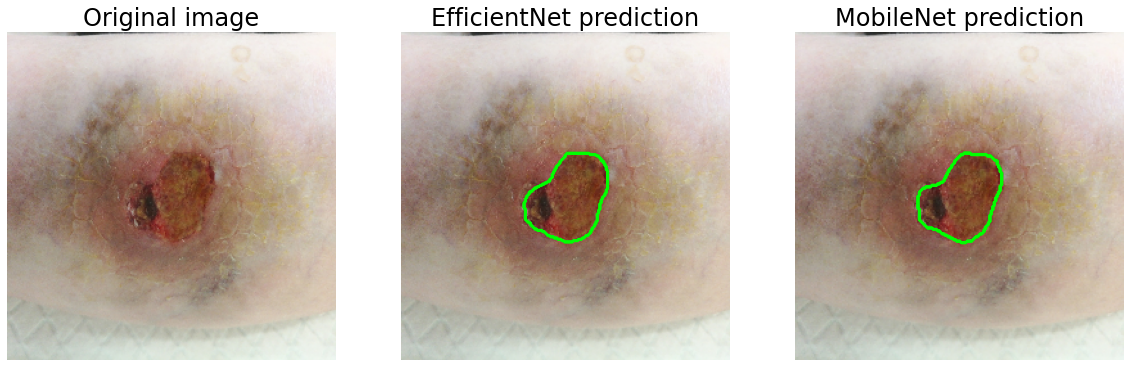
\includegraphics[clip,width=\columnwidth]{images/output-deepskin.png}%
}

\subfloat[]{%
  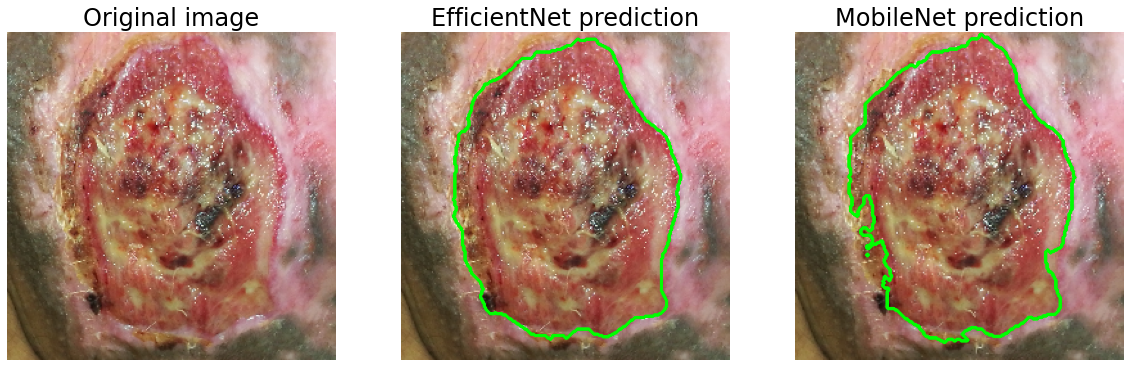
\includegraphics[clip,width=\columnwidth]{images/output2-deepskin.png}%
}

\subfloat[]{%
  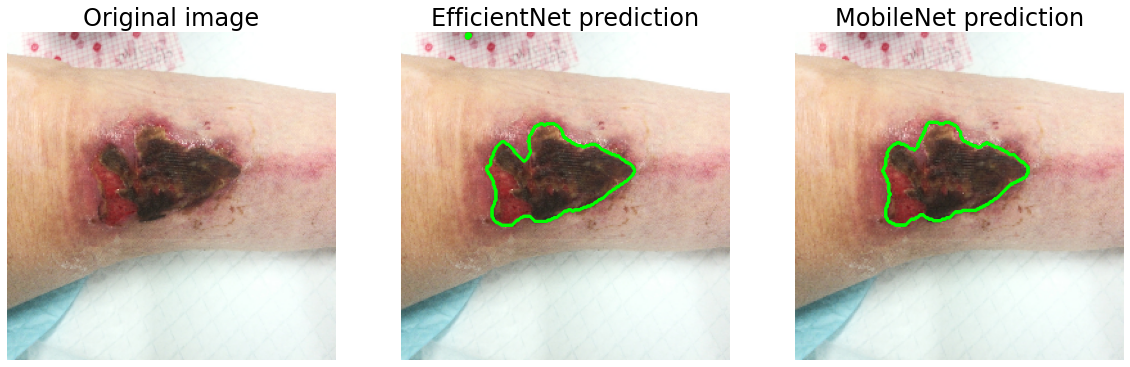
\includegraphics[clip,width=\columnwidth]{images/output3-deepskin.png}%
}
\caption{Representation of EfficientNet and MobileNet prediction on  Deepskin dataset. In (a) both modes are able to predict the same mask for the wound. In (b) MobileNet model performs worst on border detection. In (c) EfficientNet model overfits the image, recognising some background pixels as wound ones.}
\label{fig:deep-visual-results}
\end{figure}



\section{Results on PetWound}
\subsection{EfficientNet}
The application of TL was done using the EfficientNet U-Net model  pre-trained on the Deepskin dataset to predict segmentation on Petwound. This procedure resulted in a total of 143 (49\% of the whole dataset) correctly annotated images in Petwound dataset. 
This core set of images (identified as Round 0 of ASSL procedure) was used as a kick-start for the ASSL training strategy.
For each round we reported the number of images used for the training and validation of the model, the number of correctly annotated images, and the segmentation metric scores. We considered as Round 0 the one performed with the model trained only on the Deepskin dataset.
The metric scores are calculated on validation images, which were correctly segmented the previous round. 
Such score are ensuring the model performances among the rounds and we expect them to be almost constant.
\hspace{-1cm}
\begin{table}[H]
    \centering
       \scalebox{0.85}{
    \begin{tabular}{c|c|c|c|c|c|}
    
        \textbf{} & \textbf{Round 1} & \textbf{Round 2} & \textbf{Round 3} & \textbf{Round 4} & \textbf{Round 5 } \\ \hline
        \textbf{N° training images} & 127 (88\%) & 155 (86.5\%) & 170 (87.5\%) & 197 (88.2\%) & 203 (88.5\%)  \\ \hline
        \textbf{N° validation images} & 16 (12\%) & 24 (13.5\%) & 24 (12.5\%) & 24 (10.8\%) & 24 (10.5\%)  \\ \hline
        \textbf{N° correct segmentation} & 179 (62\%) & 194 (67\%) & 221 (76\%) & 227 (78\%) & 232 (80\%)  \\ \hline
        \textbf{$F_1$ score} & 0.98 & 0.98 & 0.98 & 0.98 & 0.98  \\ \hline
        \textbf{IoU score} & 0.95 & 0.96 & 0.96 & 0.96 & 0.96  \\ \hline
    \end{tabular}
    }
    \caption{Results obtained by the EfficientNet model in the ASSL training strategy on the PetWound dataset. For each round we reported the number of images used for the training and validation of the model, the number of correctly annotated images, and the segmentation metric scores. 
    We considered as Round 0 the one performed with the model trained only on the Deepskin dataset.
    The metric scores are calculated on validation images, which were correctly segmented the previous round. 
Such score are ensuring the model performances among the rounds and we expect them to be almost constant.}
    \label{tab:results-eff-petwound}
\end{table}

The best metric results of the final round of ASSL, calculated on the validation set, are reported in Table \ref{tab:results-eff-score-petwound}.
\begin{table}[H]
    \centering
    
    \begin{tabular}{|l|l|}
    \hline
          IoU  & $F_1$  \\ \hline
        0.96 & 0.98 \\ \hline
    \end{tabular}
    \caption{Results obtained by the EfficientNet after four round of ASSL. The score are calculated on the validation set.}\label{tab:results-eff-score-petwound}
\end{table}

\subsection{MobileNet}
Similarly, the application of the human pre-trained MobileNet U-Net model on the raw PetWound dataset leads to the correct annotation of 113 images (39\% of the whole dataset) thanks to TL. This core set of images was used as a kick-start for the ASSL training strategy for a total of four rounds of training.
For each round we reported the number of images used for the training and validation of the model, the number of correctly annotated images, and the segmentation metric scores. We considered as Round 0 the one performed with the model trained only on the Deepskin dataset.
The metrix scores are calculated on validation images, which were correctly segmented the previous round. 
Such score are ensuring the model performances among the rounds and we expect them to be almoast constant.
\begin{table}[H]
    \centering
    \begin{tabular}{c|c|c|c|c|}

        \textbf{} & \textbf{Round 1} & \textbf{Round 2} & \textbf{Round 3} & \textbf{Round 4 } \\ \hline
        \textbf{N° training images} & 97 (86\%) & 119 (88\%) & 122 (88.5\%) & 127 (88.5\%)  \\ \hline
        \textbf{N° validation images} & 16 (14\%) & 16 (12\%) & 16 (11.5\%) & 16 (11.5\%)  \\ \hline
        \textbf{N° correct segmentation} & 135 (47\%) & 138 (48\%) & 143 (49\%) & 145 (50\%)  \\ \hline
        \textbf{$F_1$ score} & 0.97 & 0.92 & 0.93 & 0.94  \\ \hline
        \textbf{IOU score} & 0.94 & 0.85 & 0.87 & 0.89  \\ \hline
    \end{tabular}
    \caption{Results obtained by the MobileNet U-Net model in the ASSL training strategy on the PetWound dataset.
    For each round we reported the number of images used for the training and validation of the model, the number of correctly annotated images, and the segmentation metric scores. 
    We considered as Round 0 the one performed with the model trained only on the Deepskin dataset.
The metrix scores are calculated on validation images, which were correctly segmented the previous round. 
Such score are ensuring the model performances among the rounds and we expect them to be almoast constant.}
    \label{tab:results-mob-petwound}
\end{table}

We stopped the ASSL training strategy after four rounds of training because the model performances reached a plateau. The MobileNet U-Net model did not achieve results compatible with the EfficientNet one, showing a significant gap in terms of corrected segmentation images. Despite the introduction of the TL, the lighter model was not able to generalize on the heterogeneous PetWound dataset. These results confirmed the need of a deeper or more complex model for the usage of the ASSL training strategy.

\subsubsection{MobilNet training on EfficientNet annotated images}
Since the ASSL training did not achieve the expected results, the MobileNet U-Net was then trained on the final set of annotations produced by the EfficientNet U-Net model, obtaining good results in terms of segmentation metrics (Table \ref{tab:results-mob-score-petwound-noassl}).
Such training allowed the model to reach 72\% of corrected segmentations on the whole dataset.
\begin{table}[H]
    \centering
    
    \begin{tabular}{|l|l|}
    \hline
          IoU  & $F_1$  \\ \hline
        0.90 & 0.95 \\ \hline
    \end{tabular}
    \caption{Results obtained by the MobileNet model trained on the labels segmented by EfficientNet. The metrics scores are calculated on the validation set.}\label{tab:results-mob-score-petwound-noassl}
\end{table}
\subsection{Predictions}

As we can see in Table \ref{tab:results-eff-petwound} the most significant improvement in terms of number of correct segmentation is performed between Round 0 (143 images correctly segmented via TL) and Round 1 (173 images predicted after first training on Petwound).
However, the EfficientNet model keeps improving during each round, refining step by step its predictions.
In Figure \ref{fig:pet-visual-results1} and Figure \ref{fig:pet-visual-results2} the most significant changes during ASSL training procedure are reported.

The improvement of the performances can be categorized in different sets:
\begin{itemize}
    \item the segmentation of the whole wound area from a small fraction (Figure \ref{fig:pet-visual-results1}a and Figure \ref{fig:pet-visual-results1}b);
    \item the deletion of spurious parts belonging to the background (Figure \ref{fig:pet-visual-results2}a) or to other anatomical regions (Figure \ref{fig:pet-visual-results2}b);
    \item the precise recognition of the borders (Figure \ref{fig:pet-visual-results2}c);
\end{itemize}

\begin{figure}[H]
\centering
\subfloat[]{%
  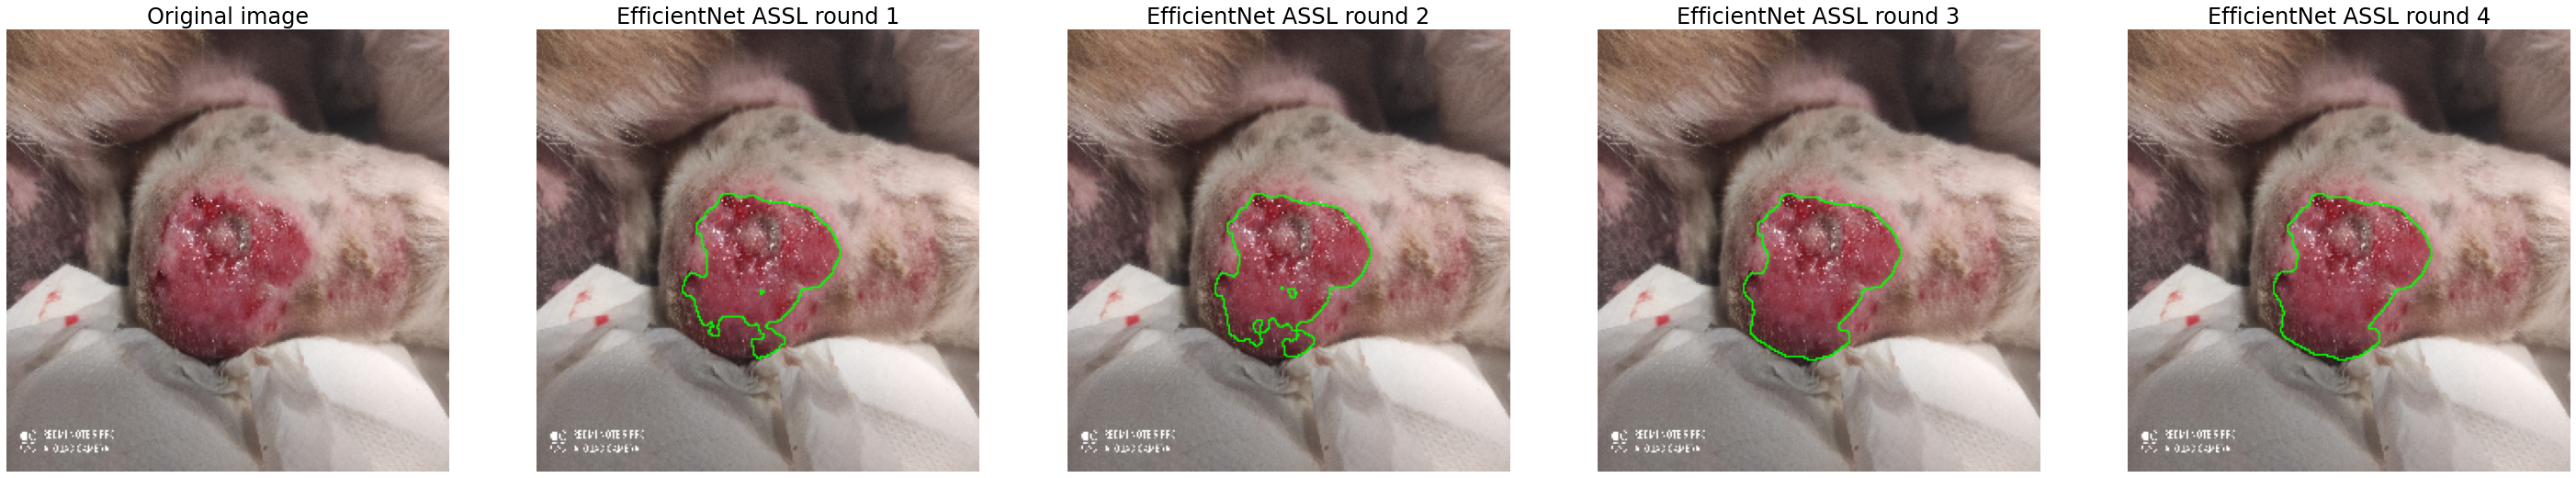
\includegraphics[width=0.2\textwidth ]{images/output_pets.png}%
}
\hspace{2cm}
\subfloat[]{%
  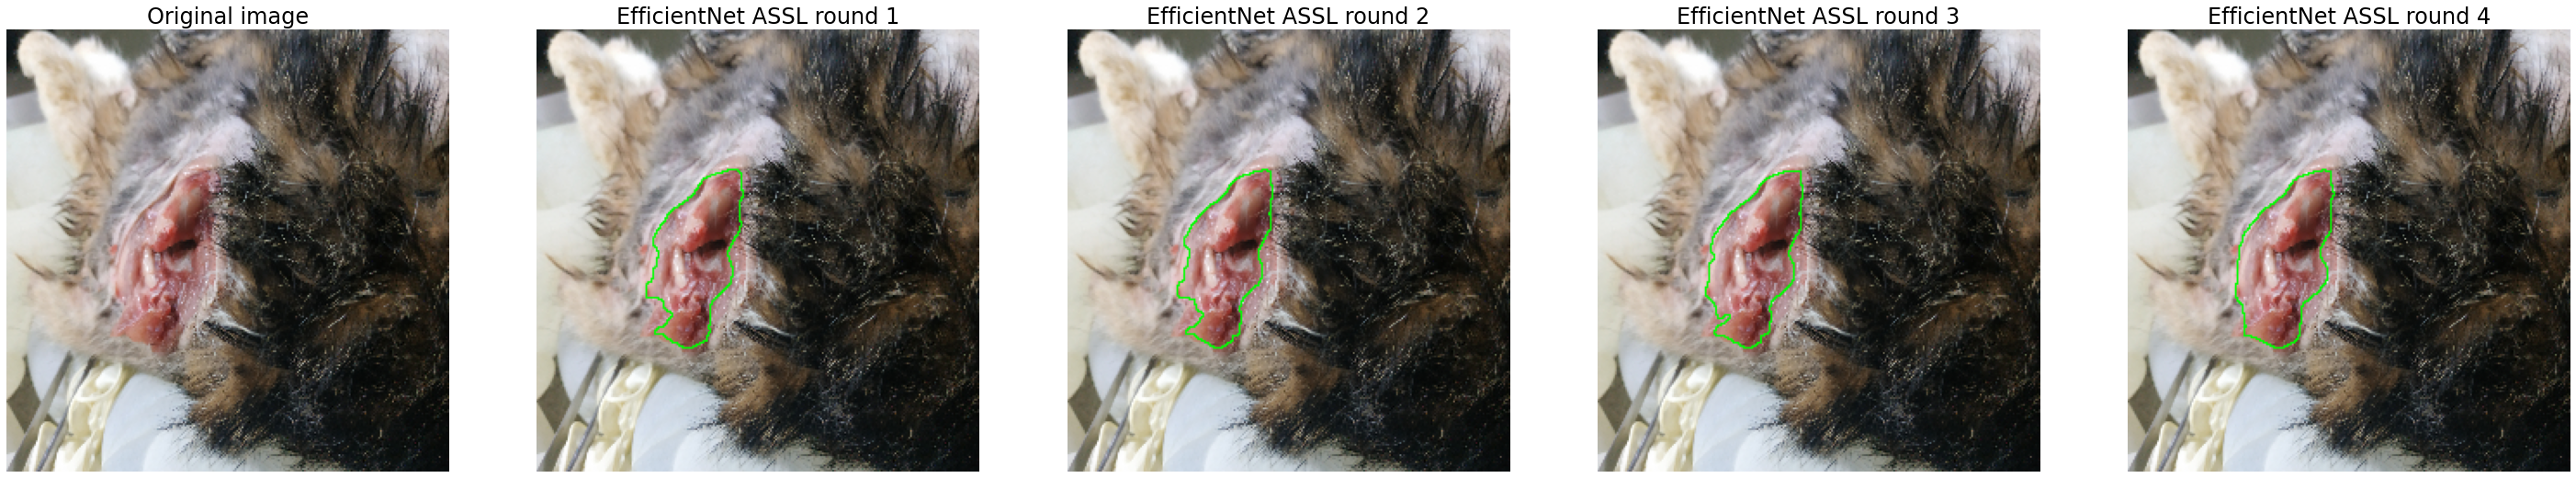
\includegraphics[ width=0.2\textwidth]{images/output3_pets.png}%
}
\caption{Evolution of EfficientNet predictions through each round on Petwound dataset. We report examples where the segmentation of the whole wound area is reached from a small fraction.}
\label{fig:pet-visual-results1}
\end{figure}

\begin{figure}[H]
\centering
\subfloat[]{%
  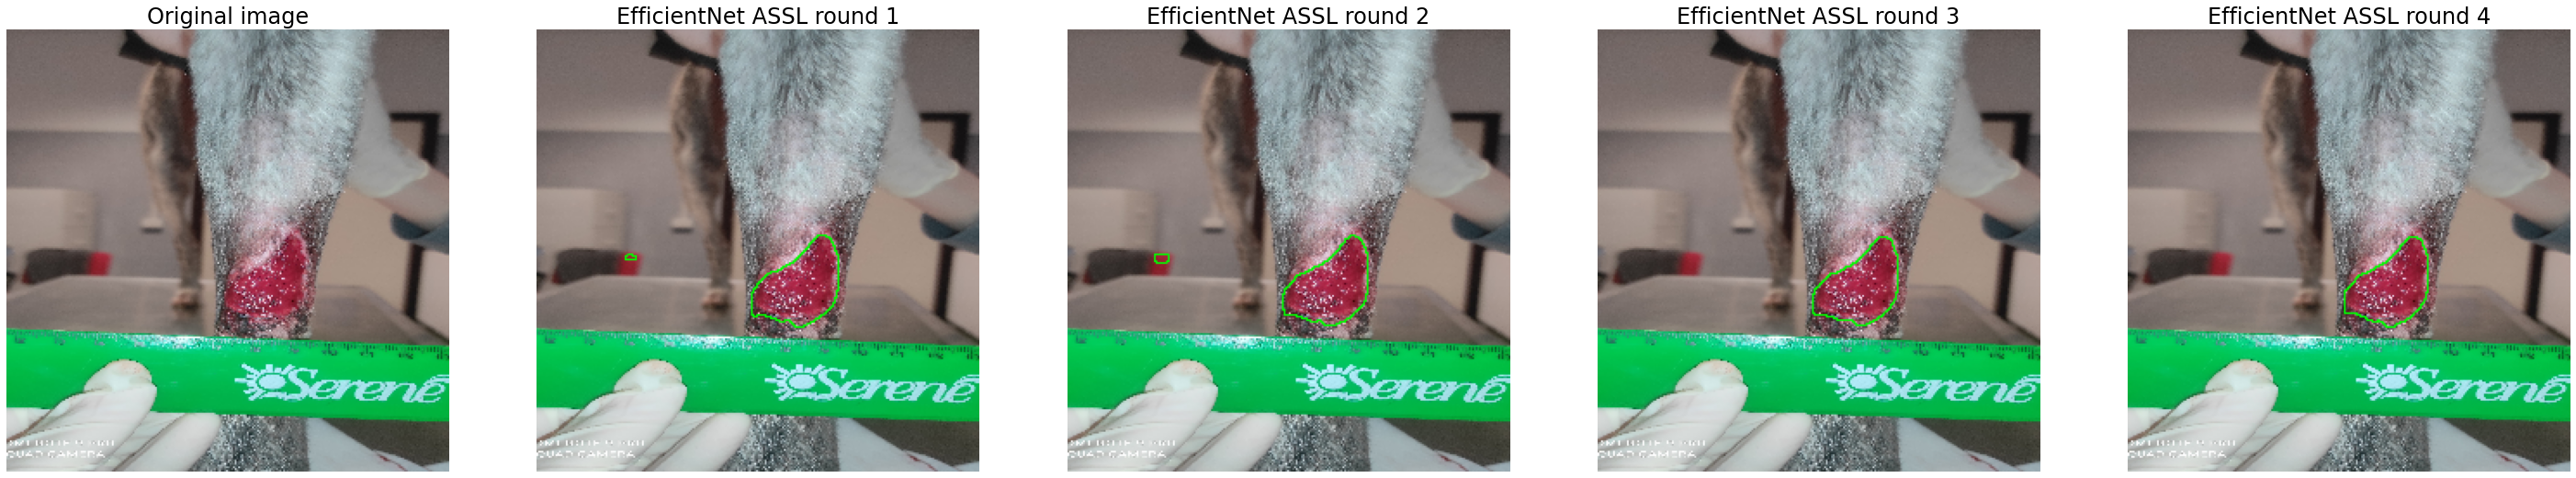
\includegraphics[width=0.2\textwidth ]{images/output2_pets.png}%
}
\hspace{2cm}
\subfloat[]{%
  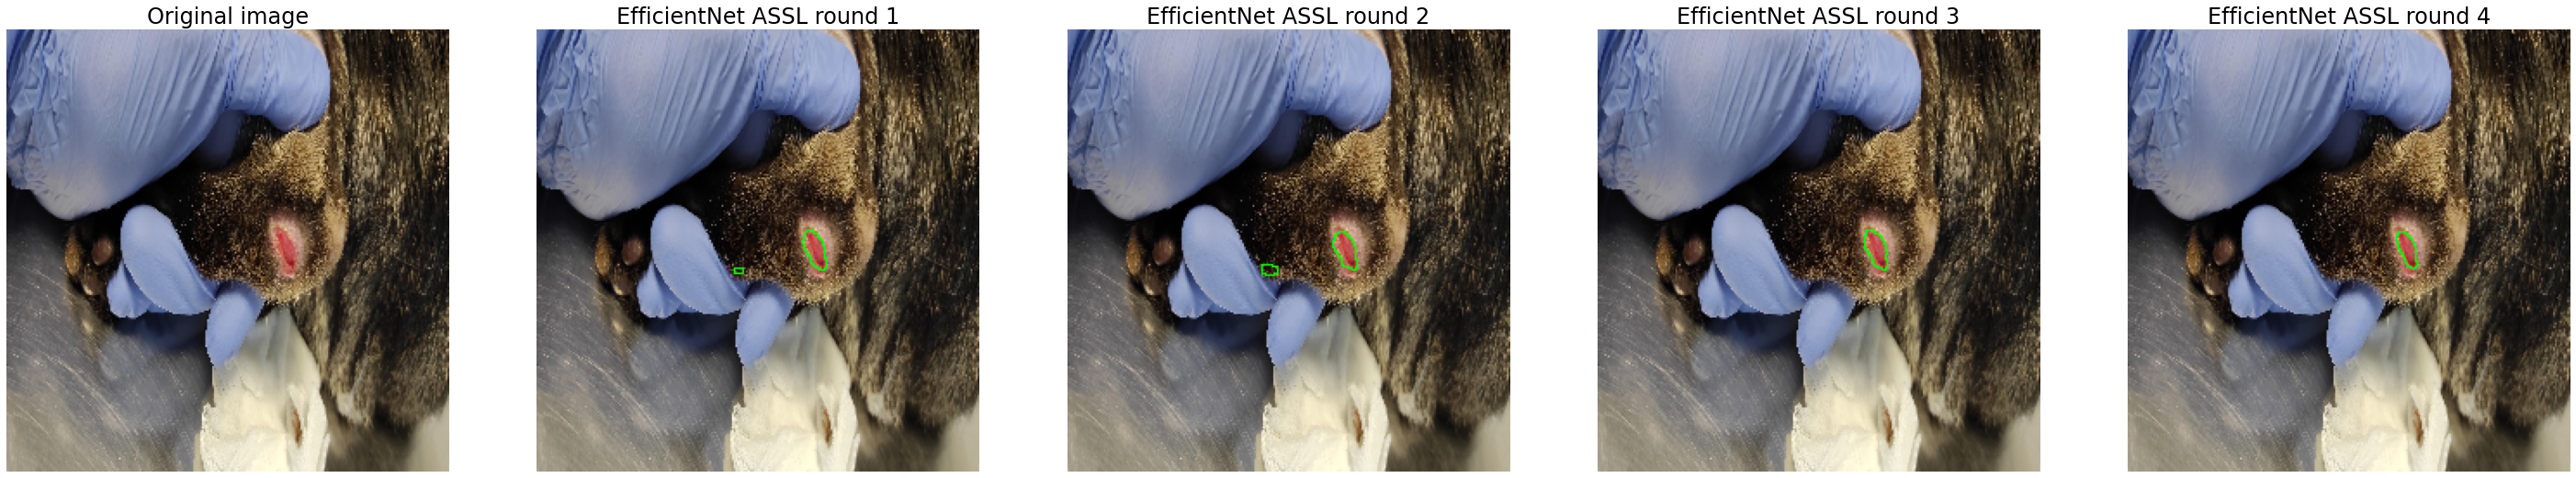
\includegraphics[width=0.2\textwidth ]{images/output4_pets.png}%
}
\hspace{2cm}
\subfloat[]{%
  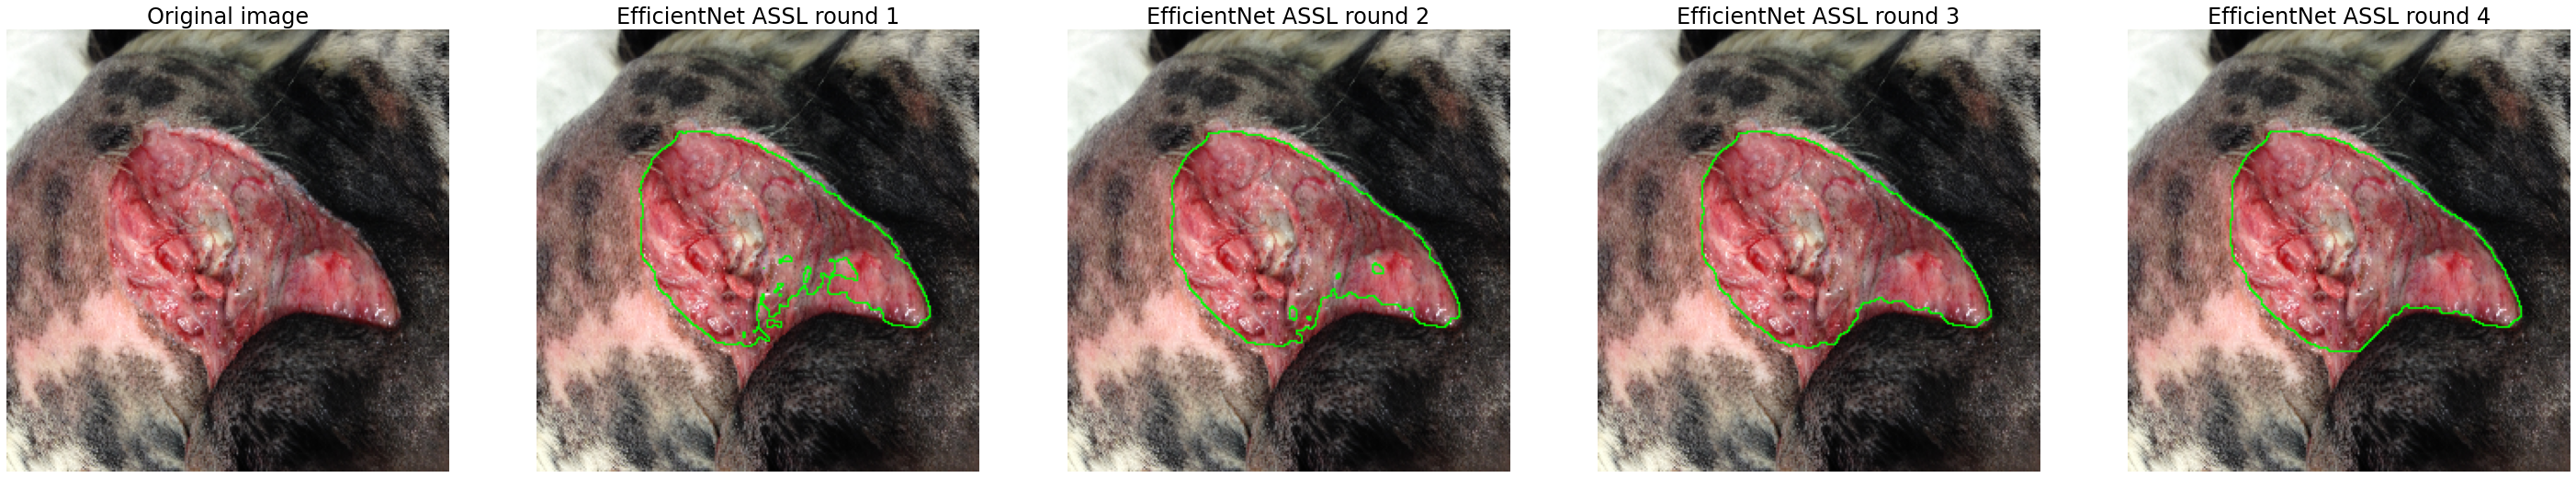
\includegraphics[width=0.2\textwidth ]{images/output5_pets.png}%
}
\caption{Evolution of EfficientNet predictions through each round on Petwound dataset. The segmentation improves by the deletion of background (a) or of other anatomical regions (b) and by reconstruction of borders (c).}
\label{fig:pet-visual-results2}
\end{figure}

\end{document}